\documentclass[a4paper]{article}


\usepackage{alphabeta} 
\usepackage{enumitem} 
\usepackage{mathtools}
\usepackage{amsmath, amssymb} 
\usepackage{amsthm}
\usepackage{cancel} 
\usepackage[margin=0.70in]{geometry} 
\geometry{left=3cm,right=3cm,top=2.4cm,bottom=2.4cm}	%the page geometry as defined, A4=210x297mm
\usepackage{graphicx}
\usepackage{wrapfig}
\usepackage{caption}
\usepackage{textcomp}
\usepackage{tabto}
\usepackage{layout}
\usepackage{bm}
\usepackage{minipage-marginpar}
\usepackage[dvipsnames]{xcolor}
\usepackage{hyperref}
\usepackage{dutchcal}
\usepackage{derivative}
\usepackage{esint}
%\usepackage{biblatex}
\usepackage{subcaption}
\usepackage{booktabs}\usepackage{derivative}
\usepackage[flushleft]{threeparttable}
\usepackage[capbesideposition=outside,capbesidesep=quad]{floatrow}
\usepackage{derivative}

%%RENEW

\newtheorem{problem}{Άσκηση}
\newtheorem*{solution*}{Λύση}
\newtheorem{definition}{Ορισμός}[subsection]
\newtheorem{properties}{Ιδιότητες}[subsection]
\newtheorem{theorem}{Θεώρημα}[subsection]
\newtheorem{protash}{Πρόταση}[subsection]
\newtheorem{porisma}{Πόρισμα}[subsection]
\newtheorem{lemma}{Λήμμα}[subsection]
\newtheorem*{prooof}{Απόδειξη}
\newtheorem*{notes}{Παρατηρήσεις}
\newtheorem*{note}{Παρατήρηση}
\newtheorem*{app}{Εφαρμογή} 
\newtheorem*{example}{Παράδειγμα}
\newtheorem*{examples}{Παραδείγματα}


\newcommand\numberthis{\addtocounter{equation}{1}\tag{\theequation}}
%\renewcommand{\labelenumi}{\roman{enumi}}
\newcommand{\approxtext}[1]{\ensuremath{\stackrel{\text{#1}}{\approx}}}
\renewcommand{\figurename}{Εικόνα.}
\renewcommand{\tablename}{Πίνακας.}
%\renewcommand\refname{New References Header}
\renewcommand*\contentsname{Περιεχόμενα}



\begin{document}
\begin{titlepage}			%makes a title page. Remember to change the author, CID, username and group number to what is appropriate for you!
	\centering
	{\scshape\LARGE Εθινικό Μετσόβιο Πολυτεχνείο\par}
	{\scshape \LARGE Σ.Ε.Μ.Φ.Ε.\par}
	\vspace{1cm}
	{\huge\bfseries Κβαντομηχανικό Φαινόμενο Σήραγγας\par}
	\vspace{1cm}
	{\Large\itshape Θωμόπουλος Σπύρος\par}		%remember to change these!
	
	%		{\large Group \@group\unskip\strut\par}
	{\large A.M ge19042 \hfill \\}% spyros.thomop@gmail.com/ ge19042@mail.ntua.gr\par		%remember to change these!
	\vspace{1cm}
	{\large 08/11/2021\par}
\end{titlepage}


\newpage 

\subsection*{Σκοπός}
Ο στόχος αυτής της εργαστηριακής άσκησης είναι η μελέτη του κβαντομηχανικού φαινομένου σήραγγας.
% Αυτό θα επιτευγχθεί μέσω της μελέτης της ψυχρής εκπομπής, αφού αποτελεί την ερμηνεία αυτής και του νόμου Fowler-Nordheim που την διέπει.
	 Συγκεκριμένα θα μελετήσουμε το φαινόμενο της ψυχρής εκπομπής ηλεκτρονίων από Βολφράμιο και τον νόμο Fowler-Nordheim που το διέπει, των οποίων εξήγηση είναι το φαινόμενο σήραγγας.
\subsection*{Θεωρητικά Στοιχεία}
\subsubsection*{Φαινόμενο Σήραγγας}
\begin{wrapfigure}{r}{0.4\textwidth}
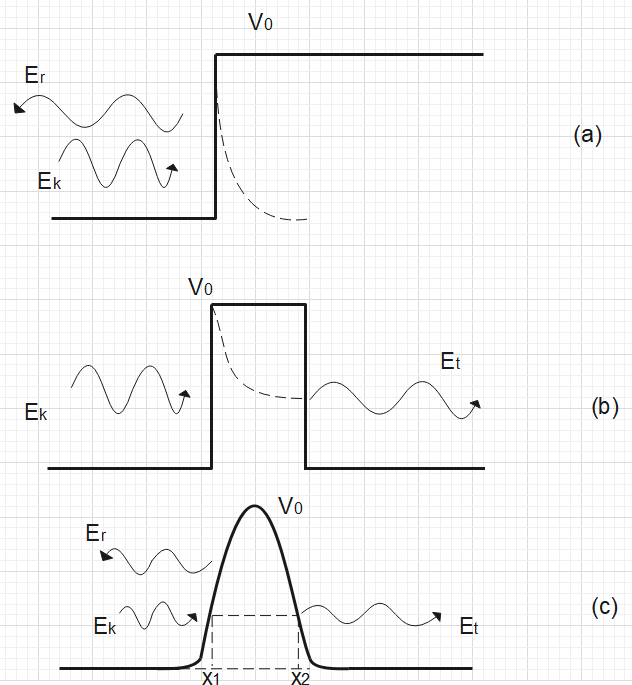
\includegraphics[width=0.9\linewidth]{tunneling.png} 
\caption{ }
\label{fig:wrapfig}
\end{wrapfigure}
Στην κβαντομηχανική, σε αντίθεση με την κλασική μηχανική, όταν ένα σωματίδιο συγκεκριμένης ενέργειας $E_k$ προσπίπτει σε ένα φράγμα δυναμικού μεγαλύτερης ενέργειας $V_0$, δεν είναι βέβαιο ότι θα ανακλαστεί. 
Όταν πρόκειται για δυναμικό άπειρου ύψους, μόνο τότε οι δύο θεωρίες συμφωνούν, το σωματίδιο δεν εισέρχεται στην περιοχή του δυναμικού και ανακλάται πλήρως. 
Ωστόσο, όταν το δυναμικό έχει πεπερασμένο ύψος αλλά και άπειρο πλάτος (σκαλοπάτι δυναμικού, Εικόνα 1.α), υπάρχει μία πιθανότητα διείσδυσης εντός της κλασικά απαγορευμένης περιοχής του δυναμικού, η οποία φθίνει εκθετικά με την απόσταση.
 Ακόμη, όταν το δυναμικο εκτός από πεπερασμένο ύψος $V_0$ έχει και πεπερασμένο πλάτος $L$ (φράγμα δυναμικού Εικόνες 1.b,c), το σωματίδιο "χωρίζεται". Ένα μέρος του διέρχεται μέσα από το φράγμα και εν τέλει μειώνεται η ενέργειά του, ενώ ένα άλλο μέρος ανακλάται. Αυτό είναι ποιοτικά το \textit{ Κβαντομηχανικό Φαινόμενο Σήραγγας}. Από τα δύο τελευταία φαινόμενα αναδύεται και η κυματική φύση των σωματιδίων στην Κβαντομηχανική θεωρία.

Για να διέλθει το σωματίδιο από το φράγμα δυναμικού και να παρατηρηθεί το φαινόμενο σήραγγας, το πλάτος του φράγματος θα πρέπει να είναι της τάξης του μήκους κύματος De Broglie του σωματιδίου που αντιστοιχεί στην ενέργεια που κατέχει. Στην	πρείπτωσή μας, θα έχουμε ηλεκτρόνια με την ενέργεια Fermi του Βολφραμίου, δηλαδή $5.7eV$, που αντιστοιχεί σε $\simeq 5.1 \mathring{A}$.

Ποσοτικά, το φαινόμενο φράγματος περιγράφεται από τους συντελεστές διάδοσης $Τ(Ε_κ)$ και ανάκλασης $R(E_k)$\footnotemark, οι οποίο εκφράζουν αντίστοιχα την πιθανότητα διέλευσης και ανάκλασης μίας δέσμης όμοιων σωματιδίων.%όταν έχουμε σωματίδια ίδιας μάζαςτου σωματιδίου.
% ή αλλίως σε μία πίο "κυματική" περιγραφή το ποσοστό του σωματιδίου να διέλθει και ναι ανακλαστεί από το φράγμα. 
\footnotetext{Από την σχέση $R(E_k)+T(E_k)=1$ εκφράζεται και η διατήρηση της ενέργειας.}
Ο συντελεστής διάδοσης που μας ενδιαφέρει σε αυτή την πειραματική άσκηση είναι 
\begin{equation}
T(E_k) = \frac{J_{in}}{J_{t}}
\end{equation}
όπου $J_{in}$ και $J_{t}$ είναι αντίστοιχα τα ρεύματα πιθανότητας της προσπίπτουσας και της δερχόμενης δέσμης ηλεκτρονίων. 

Από την εξίσωση Scrodinger
\begin{equation}
-\frac{\hbar ^2}{2m}\pdv[2]{\Psi(x)}{x} + V(x) \Psi(x) = E \Psi(x)
\end{equation}
σε συνδυασμό με την σχέση για το ρεύμα πιθανότητας 
\begin{equation}
J = -i\frac{\hbar}{2m}(\Psi^*\pdv{\Psi}{x} - \Psi\pdv{\Psi^*}{x})
\end{equation}
και τις συνοριακές συνθήκες συνέχειας της κυματοσυνάρτησης και της παραγώγου της στις διαδοχικές περιοχές αλλαγής δυναμικού, για το \underline{ορθογώνιο φράγμα} προκύπτει ότι ο συντελεστής διέλευσης είναι: 
\begin{align*}
T(E_k) &= \left( 1 + \frac{sinh^2(k_2 L)}{4\frac{E_k}{V_0}(1-\frac{E_k}{V_0})} \right)^{-1} \stackrel{k_2L>>1}{\simeq} \footnotemark  
\left( 1 + \frac{e^{2k_2 L}}{16\frac{E_k}{V_0}(1-\frac{E_k}{V_0})} \right)^{-1} \Rightarrow \\ 
&\simeq 16\frac{E_k}{V_0}\left(1-\frac{E_k}{V_0}\right)e^{-2k_2 L}  \numberthis %\label{eqn}
\end{align*}

όπου $k_2:=\sqrt{ 2m(V_0-E_k)/\hbar^2}$. \\
\footnotetext{Έχουμε $sinh(k_2 L) = 1/2(e^{k_2L} - e^{-k_2L}) \simeq  e^{k_2 L}/2$} 
\newpage
Είναι εμφανές πως ο συντελεστής διέλευσης έχει ισχυρή εξάρτηση κυρίως από την τιμή του $k_2$.
Κατ' αναλογία, αν το δυναμικό δεν έχει σταθερή τιμή $V_0$ αλλά είναι $V=V(x)$, τότε θα μεταβάλλεται το $k_2$ συνεπώς στην τελεταυταία σχέση αντικαθιστούμε το $k_2$ από την μέση τιμή του για το χωρικά μεταβαλλόμενο δυναμικό
\begin{equation}
\left<k_2(x)\right> = \frac{1}{L} \int_{x_1}^{x_2}{ \sqrt{\frac{2m}{\hbar^2}\left(V(x)-E_k)\right)}dx}
\end{equation}
%από την προσέγγιση $JWKB$, απλώς αντικαθιστούμε τοο σταθερό δυναμικό με την συνάρτηση δυναμικού στην τελευταία σχέση () και προκύπτει
όπου πλέον $L=x_2-x_1$ όπως φαίνεται στην Εικόνα 1.c, με $x_1,x_2$ να 'ναι τα όρια της κλασικά απαγορευμένης περιοχής  που αντιστοιχεί στην ενέργεια του ηλεκτρονίου. Έτσι, προκύπτει ο συντελεστής διέλευσης από την προσέγγιση $JWKB$ 
\begin{equation}\label{6}
T(E_k)\simeq 16\frac{E_k}{V_0}\left(1-\frac{E_k}{V_0}\right) e^{-2\left<k_2\right> L}
\end{equation}
Μπορούμε να παρατηρήσουμε πως όσο μικραίνει το πλάτος του φράγματος στην εκάστοτε ενεργειακή στάθμη, μεγαλώνει η τιμή του συντελεστή διέλευσης, άρα είναι πιό πιθανό να διέλθουν κάποια σωματίδια από την δέσμη.

\subsubsection*{Μοντέλο Μετάλλου}
Για τα μέταλλα θα χρησιμοποιήσουμε το μοντέλο των ελεύθερων ηλεκτρονίων του Sommerfeld, σύμφωνα με το οποίο, τα ηλεκτρόνια του μετάλλου που προκαλούν την ηλεκτρική του αγωγιμότητα είναι ελεύθερα, μη αλληλεπιδρώντα και σε πρώτη φάση περιλαμβάνει το γεγονός ότι έχουν διακριτές ενέργειες και ότι είναι φερμιόνια, δηλαδή ακολουθούν την στατιστική Fermi-Dirac και υπόκεινται στην απαγορευτική Αρχή Pauli. 

Θεωρούμε τα ηλεκτρόνια ως επίπεδα κύματα τα οποία ανακλώνται μόνο στο εσωτερικό της επιφάνειάς του. Έτσι παίρνουμε τις δέσμιες καταστάσεις, που σημαίνουν διακριτότητα για την ενέργεια.
% Οι εν λόγω καταστάσεις χαρακτηρίζονται από μεγάλη πυκνότητα και γι' αυτό μπορούμε να θεωρήσουμε το φάσμα της ενέργειας συνεχές.
Επίσης, δεδομένου ότι στην παραπάνω ανάλυση του φαινομένου σήραγγας δεν υπεισέρχεται καθόλου η θερμοκρασία, αυτή δεν θα έχει μεγάλη επίδραση στο φαινόμενο και την θεωρούμε $Τ=0K$. Τότε, υπάρχει ένα άνω φράγμα για την 
%\textcolor{red}{απόλυτη} 
τιμή της ενέργειας που μπορούν να έχουν τα ηλεκτρόνια εντός του μετάλλου, που καλείται \textit{ενέργεια Fermi, $E_f$}. 




Μπορούμε να θεωρήσουμε το δυναμικό του μετάλλου $-V_0$ και το δυναμικό εκτός μετάλου $0$, τότε η ενέργεια Fermi είναι αρνητική, προκειμένου οι υπόλοιπες στάθμες να έχουν 
%\textcolor{red}{κατ' απόλυτη τιμή} 
μικρότερη ενέργεια 
%αλλά η ενέργεια για την οποία το ηλεκτροόνιο εξέρχεται από το μέταλλο να 'ναι μηδενική,
έχουμε την Εικόνα 2.α.
\footnote{Στην πραγματικότητα δεν πρόκειται για σκαλοπάτι δυναμικού όπως φαίνεται στην εικόνα, αλλά για πηγάδι, διότι έτσι επιτυγχάνονται οι δέσμιες καταστάσεις.}
 Η ενέργεια Fermi δίνεται από την σχέση 
 \begin{equation}
 	E_f =\textcolor{red}{-} \frac{h^2(3\pi^2 n)^{2/3}}{8m_e\pi^2}
 \end{equation}
όπου n είναι ο αριθμός ηλεκτονίων ανά μονάδα όγκου.

Γενικα, είναι γνωστό από την Μηχανική, ότι σε εναν στοιχειώδη όγκο dV ενός δεδομένου στερεού θα υπάρχει μία στοιχειώδης ποσότητα μάζας dm, ποσότητες που συνδέονται μέσω της πυκνότητας μάζας του στερεού $\rho(r)$, με τον εξής τρόπο: $dm=\rho(r) dV$.
%, όπου $\rho$ είναι η πυκνότητα μάζας του στερεού, μιά συνάρτηση της θέσης, r.
 Κατ' αναλογία, έχουμε ότι σε μία συγκεκριμένη στοιχιώδη περιοχή ενεργειών, πλάτους dE ( δηλαδή για ενέργειες που ανήκουν στο διάστημα $(E,E+dE)$) θα υπάρχει συγκεκριμένος αριθμός ηλεκτρονίων $dN$, που έχουν ενέργεια εντός του $(E,E+dE)$. Τα δύο αυτά μεγέθη συνδέονται μέσω της \textit{πυκνότητας ενεργειακών καταστάσεων} $\rho (E)$, σύμφωνα με την σχέση $dN=\rho(E)dV$. Ωστόσο, επειδή τα ηλεκτρόνια είναι φερμιόνια συνεπώς ακολουθούν την στατιστική Fermi-Dirac, το σύστημα δεν είναι ισοπίθανο να βρίσκεται σε κάθε ενεργειακή κατάσταση. Η κατανομή πιθανότητας δίνεται από την κατανομή Fermi-Dirac $f(E)$, δηλαδή έχουμε ότι $dN=\rho(E)f(E)dV$. Σε άλλη μορφή, έπειτα από την αντικατάσταση της συνάρτησης κατανομής $f(E)$, γράφεται: 
\begin{equation}
\rho(E)f(E) = \frac{8\pi}{h^3}\sqrt{2m_e^3}\frac{\sqrt{E}}{\exp{(E-|E_f|)kT}+1}
\end{equation}
\newpage
Ακόμη, δεν έχει γίνει ξεκάθαρος ο λόγος για τον οποίον θεωρούμε την ενέργεια Fermi αρνητική. Προκειμένου να ξεφύγουν τα ηλεκτρόνια απ' το σκαλοπάτι δυναμικού,
\footnote{Ξανατονίζω ότι το σκαλοπάτι δεν είναι η κατάλληλη ονομασία καθώς δεν δίνει δέσμιες καταστάσεις. Στην πραγματικότητα πρόκειται για πηγάδι.} 
θα πρέπει να έχουν μεγαλύτερη ενέργεια από το ύψος του σκαλοπατιού, πράγμα αδύνατο καθώς είναι παγιδευμένα μεσα στο μέταλλο. Ωστόσο, μπορούμε να τα απεγκλωβίσουμε, είτε προσφέροντάς τους ενέργεια φ (έργο εξόδου), ώστε να υπερπηδήσουν το φράγμα, είτε αν με κάποιον τρόπο μετατρέψουμε το πλάτος του σκαλοπατιού από άπειρο σε πεπερασμένο (φράγμα δυναμικού). Τότε τα ηλεκτρόνια θα μπορούν να το προσπεράσουν. Η εξήγηση του τελευταίου εγκειται στο φαινόμενο σήραγγας.

Αριθμητικά, για το βολφράμιο η ενέργεια Fermi είναι $|E_f|=5.7eV$ ενώ το έργο εξαγωγής, η ενέργεια δηλαδή που πρέπει να προσφέρουμε στο ηλεκτρόνιο για ξεπεράσει το δυναμικό του μετάλλου είναι $\phi=4.5eV$. Υποθετικά, αν τα ηλεκτρόνια δεν είχαν ενέργεια, τότε θα  βρίσκονταν στο δυναμικό του μετάλλου $V_0=-(5.7+4.5)=-10.2V$. Ωστόσο, αυτό είναι αδύνατο και τους "επιβάλλεται" μια ελάχιστη ενέργεια $E_f=5.7eV$ άρα 
η ενέργειά τους γίνεται $E'=-10.2eV+5.7eV=-4.5eV$, απ' όπου για να πάνε στο μηδενικό δυναμικό/μηδενική ενέργεια θα πρέπει να τους προσφερθεί ενέργεια ίση με το έργο εξαγωγής φ.
%στο δυναμικό προστίθεται η αντίστοιχη ποσότητα και γίνεται $V_0' = -10.2V+5.7V=-4.5V$, απ' όπου για να φτάσουν στο μηδενικό δυναμικό θα πρέπει να του προσφερθεί ενέργεια ίση με το έργο εξαγωγής. 
Αυτό φαίνεται στην Εικόνα 2.b.
\\
Εφαρμόζοντας ένα πολύ ισχυρό ηλεκτρικό πεδίο $F$ στην εξωτερική επιφάνεια του μετάλλου, η δυναμική ενέργεια του ηλεκτρονίου όταν βρίσκεται εκτός μετάλλου, δίνεται από την σχέση
\begin{equation}
U_d = - e F x
\end{equation}
θεωρώντας $x$ την απόσταση από την εξωτερική επιφάνεια.
Συνεπώς, το σκαλοπάτι άπειρου πλάτους μετατρέπεται σε ένα τριγωνικό φράγμα, όπως αυτό που φαίνεται στην Εικονα 2.b, το οποίο έχει μαθηματική μορφή
\begin{equation}
U(x)=U_d = -eFx %\Rightarrow \boxed{U=(\overbrace{-\phi+V_f}^{-10.2V}+eFx)V}
\end{equation}

\begin{figure}[h!]
\centering
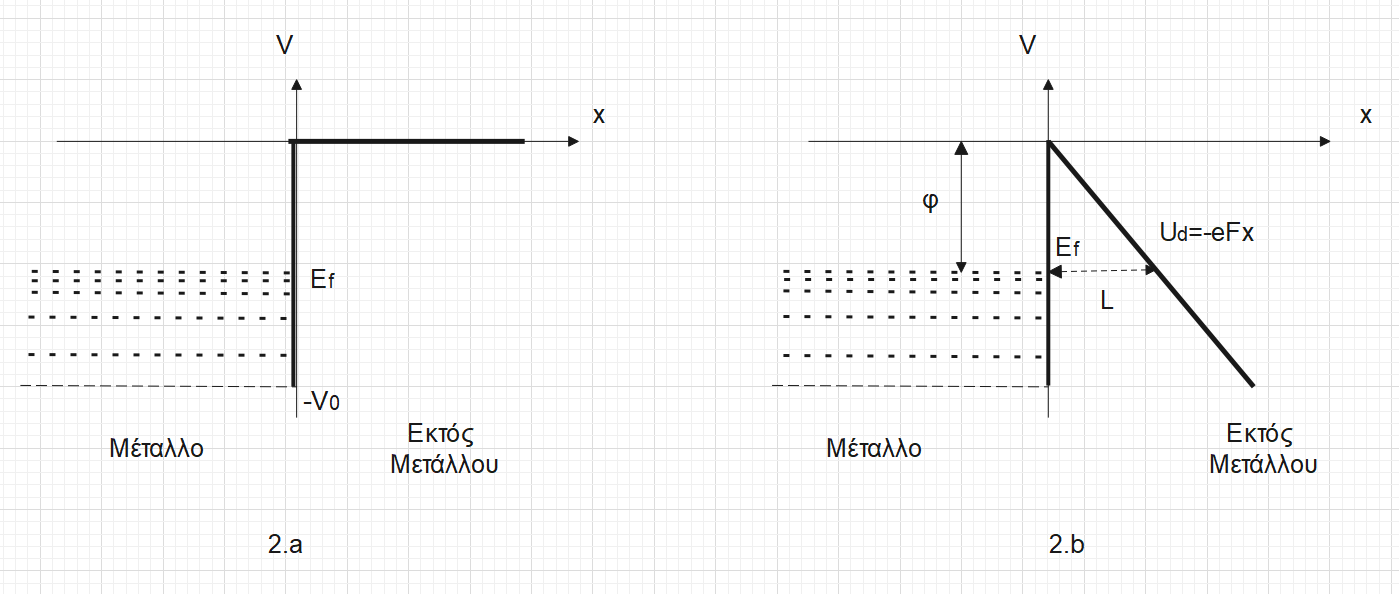
\includegraphics[scale=0.4]{poten.png}
\caption{ }
\end{figure}

Αν θεωρήσουμε L το πλάτος του φράγματος για μία συγκεκριμένη τιμή της ενέργειας, δηλαδή το πλάτος που "αντιλαμβάνεται" το ηλεκτρόνιο, τότε το έργο εξαγωγής θα είναι 
\begin{equation}
U(x)=-eFL=-\phi \Rightarrow L = \phi/eF
\end{equation}
άρα όσο μεγαλύτερο είναι το πεδίο F που εφαρμόζουμε στο μέταλλο, τόσο πίο πολύ στενεύει το φράγμα, που σημαίνει ότι ο συντελεστής διέλευσης της σχέσης (\ref{6}) μεγαλώνει τότε θα είναι πιό πιθανό για ένα ηλεκτρόνιο να εξέλθει.\footnotemark

\footnotetext{Για $T>0$  υπεισέρχεται μία διόρθωση στο μοντέλο, καθώς τα ηλεκτρόνια έχουν ενέργεια $Ε>Ε_f$ και "βλέπουν" μικρότερο πλάτος στο φράγμα, άρα είναι πιό πιθανό να εξέλθουν λόγω του φαινομένου σήραγγας. Ακόμη. αγνοήσαμε το φαινόμενο Shottky, κατά το οποίο μειώνεται η κορυφή του δυναμικού, δηλαδή το έργο εξόδου. Ο αριθμός των ηλεκτρονίων που εξέρχονται από αυτά τα δύο φαινόμενα είναι αμελητέος, ενδεχομένως μη ανιχνεύσιμος από την διάταξή μας, και γι' αυτό μπορούμε να τα αγνοήσουμε.}

Πιό συγκερκιμένα, το μέταλλο που χρησιμοποιούμε είναι ένα σύρμα βολφραμίου μεγάλης καμπυλότητας (συγκεκριμένα πρόκειται για παραβολοειδές) προκειμένου για τάσεις της τάξης $3-10kV$ να παράγονται ισχυρά ηλεκτρικά πεδία στην κορυφή του. Για τον ποιοτικό έλεγχο της θεωρίας θα έχουμε 
\begin{equation}\label{12}
%F=\frac{V}{r}\frac{2}{ln(2R/r)}
F=\xi V
\end{equation}
όπου  $\xi=\frac{1}{r}\frac{2}{ln(2R/r)}$ και περιλαμβάνει τα γεωμετρικά χαρακτηριστικά της ακίδας. Ισχύει ότι $R=0.04m$ και είναι η απόσταση ακίδας-συλλέκτη ηλεκτρονίων.
Επίσης στην κορυφή συμβαίνει το φαινόμενο σήραγγας που περιέγραψα παραπάνω.


Η ένταση του ρεύματος αυτών των ηλεκτρονίων που εξέρχονται λόγω της ψυχρής εκπομπής γενικά θα είναι της μορφής 
\begin{align*}\label{13}
%J_e=P\frac{e^2}{2\pi h}\frac{F^2}{\phi}exp\left(-\frac{8\pi\sqrt{2}\phi^{3/2}}{2\pi heF}\right)
%J_e=CF^2exp\left(-\frac{B}{F}\right)
I_{cold}&=CV^2exp\left(-\frac{B}{V}\right) \xRightarrow{ln} \\ 
ln(I_{cold}/V^2)&=lnC-B/V \numberthis
\end{align*}
%Το $P$ είναι μία σταθερά του μετάλλου, η οποία εν γένει εξαρτάται από το δυναμικό $Fermi V_f$ και το έργο εξόδου, η οποία στην περίπτωση του βολφραμίου είναι $P=1.12\sqrt{V}$.
Τα $C,B$ είναι σταθερές που στην περίπτωση του νόμου Fowler-Nordheim είναι
\begin{align*}\label{14}
%B=\frac{8\pi\sqrt{2m}\phi^{3/2}}{2\pi he}6.827\times10^{9} \phi^{3/2}\\
%C=P\frac{e^2}{2\pi h}\frac{1}{\phi}=0.06168\frac{P}{\phi}
B=\frac{6.83\times10^9\phi^{3/2}}{\xi}, \text{       }[V]          \numberthis      \\
C=\frac{SP\xi^2\times10^{-2}}{\phi},\text{         }[AV^{-2}]      \numberthis
\end{align*}
Το $P$ είναι μία σταθερά του μετάλλου, η οποία εν γένει εξαρτάται από το δυναμικό $Fermi \text{ } V_f$ και το έργο εξόδου. Στην περίπτωση του βολφραμίου είναι $P=1.12\sqrt{V}$. Ακόμη, τo $S$ είναι η μέση επιφάνεια της ακίδας.

Άρα περιμένουμε ότι αν μετρήσουμε το ρεύμα ψυχρής εκπομπής $I_{cold}$ στην κορυφή της ακίδας συναρτήσει της εφαρμοζόμενης διαφοράς δυναμικού, θα επαληθευτεί ο νόμος Fowler-Nordheim, (\ref{13}).

\subsection*{Πειραματική Διάταξη}

Η πειραματική διάταξη αποτελείται από
\begin{itemize}
\item[.] \textit{Λυχνία-δίοδος κενού} μέσα στην οποία υπάρχει ένα λεπτό σύρμα από βολφράμιο, στην άκρη του οποίου βρίσκεται η ακίδα. Απέναντί της, η επιφάνεια του γυαλιού έχει επικαλυφθεί με διάφανη στρώση $SnCl_2$ που λειτουργεί ως ανιχνευτής και διοχετεύει το ρεύμα σε ηλεκτρικό κύκλωμα. Επίσης πάνω από το $SnCl_2$ υπάρχει ένα στρώμα λευκού ZnS ο οποίος αναμεμειγμενος με μερικά ppm ενός ενεργοποιού στοιχείου όπως Cu (στην περίπτωσή μας δεν ξέρουμε τί υπήρχε) γίνεται φθορίζων και μπορούμε να παρατηρήσουμε πράσινο χρώμα κατά την πρόσπτωση ισχυρής δέσμης ηλεκτρονίων σ' αυτόν.

\item[.] \textit{βάση} στην οποία τοποθετείται η λυχνία
\item[.] πηγή υψηλής τάσης
\item[.] ψηφιακό μετρητή/πολύμετρο
\item[.] αυτοσχέδιο ηλεκτρόμετρο που αυξάνει την ευαισθησία μέτρησης του ρεύματος σε κλίμακα 1-1000nA
\end{itemize} 

\subsection*{Πειραματική Διαδικάσία - Επεξεργασία Μετρήσεων}
Στις μικρές τάσεις εώς $3kV$ στο μετρούμενο ρεύμα επικρατεί η επίδραση του ρεύματος διαρροής της διάταξης το οποίο αυξάνεται γραμμικά με την τάση. Ωστόσο όπως μας λέει η σχέση (\ref{13}) το ρεύμα ψυχρής εκπομπής θα αυξάνεται εκθετικά με την τάση συνεπώς όταν αυτό κυριαρχεί η τιμή του συνολικού ρεύματος θα αυξηθεί απότομα. Για να προσδιορίσουμε την τιμή του $I_{cold}$ απλώς θα αφαιρέσουμε το ρεύμα διαρροής $I_{leak}$. 

Για να το βρούμε, σε πρώτη φάση αυξάνουμε την τάση της πηγής με βήμα $400V$ και καταγράφουμε την τάση για την οποία το ρεύμα αυξάνει απότομα. Η εν λόγω τάση βρέθηκε  
\begin{equation*}
V_{a}=(5.2\pm0.3)kV \footnotemark
\end{equation*}
\footnotetext{Το σφάλμα του βολτομέτρου της πηγής τάσης για την κλιμακα που βρισκόμαστε είναι $\pm3\%²kV$.}
%$\delta V=V\cdot0.05\%+3*10^{-4V}=0.2653\simeq 0.3 kV$} %}

%\textcolor{red}{και το αντίστοιχο ρεύμα 
%\begin{align*}
%I_{leak} = (11\pm3)nA 
%\end{align*}}



Για να βρούμε το ρεύμα διαρροής, μετράμε το ρεύμα σε τάση $V_{leak}=(V_a-0.3)kV=4.9kV$ το οποίο είναι 
\begin{equation*}
I_{leak} = (5.0\pm3.0)nA \footnotemark
\end{equation*}
\footnotetext{Το μεγάλο σχετικό σφάλμα της μέτρησης του ρεύματος διαρροής οφείλεται στην πολύ μικρή τιμή του. Στην συνέχεια το σχετικό σφάλμα της κάθε μέτρησης μειώνεται.}

Το σφάλμα για την μέτρηση του ρεύματος είναι 
\begin{equation}
\delta I = (0.01\cdot I +3 )nA
\end{equation}

Τώρα από την τάση διαρροής που βρήκαμε αυξάνουμε την τάση με βήμα $200V$ καταγράφοντας το αντίστοιχο ρεύμα $(I_1)$, το οποίο δεν θα πρέπει να ξεπεράσει τα $1000nA$ καθώς ενδέχεται να δημιουργηθούν φθορές στην ακίδα. Όταν φτάσουμε στην μέγιστη τάση επαναλαμβάνουμε τις μετρήσεις μειώνοντας την τάση κατα $200V$ σε κάθε μέτρηση (μετράμε ρεύμα $I_2$). 

Για να βρούμε το ρεύμα ψυχρής εκπομπής, παίρνουμε την μέση τιμή των $I_1,I_2$ και αφαιρούμε το ρεύμα διαρροής της διάταξης. Το αποτελέσματα φαίνονται στον Πίνακα 1. 

\begin{table}[h!]
\centering 
\caption{\textcolor{white}{.}}\footnotemark
\begin{tabular}{r|r||r|r||r|r}
$V_1(kV)$& $I_1(nA)$ & $V_2(kV)$ & $I_2(nA)$ & $I_{mean}(nA)$ & $I_{cold}(nA)$\\
\hline\hline
% 	5.2&   7.0&   5.2&   7.0&   7.0000&    
    5.4&  14.0&   5.4&  17.0&  15.5& 10.5  \\
    5.6&  31.0&   5.6&  34.0&  32.5& 27.5 \\
    5.8&  65.0&   5.8&  72.0&  68.5& 63.5\\
    6.0& 130.0&   6.0& 130.0& 130.0&125.0\\
    6.2& 283.0&   6.2& 223.0& 253.0&248.0\\
    6.4& 467.0&   6.4& 450.0& 458.5&453.5\\
    6.6& 740.0&   6.6& 747.0& 743.5&738.5\\
    6.7& 879.0&   6.7& 879.0& 879.0&874.0\\
\end{tabular}
\end{table}
\footnotetext{Πήραμε και μία μέτρηση που δεν αντιστοιχεί σε βήμα 200V για να έχουμε περισσότερες.}

Η γραφική παράσταση του $I_{cold}$ συναρτήσει του $V$ όπως προκύπτει από τα δεδομένα φαίνεται στην Εικόνα 3.\footnote{Χρησιμοποιήθηκε polynomial fit με βαθμό πολυωνύμου 3.}
\begin{figure}[h!]
\centering 
\caption{Καμπύλη $I_{cold}-V$ }
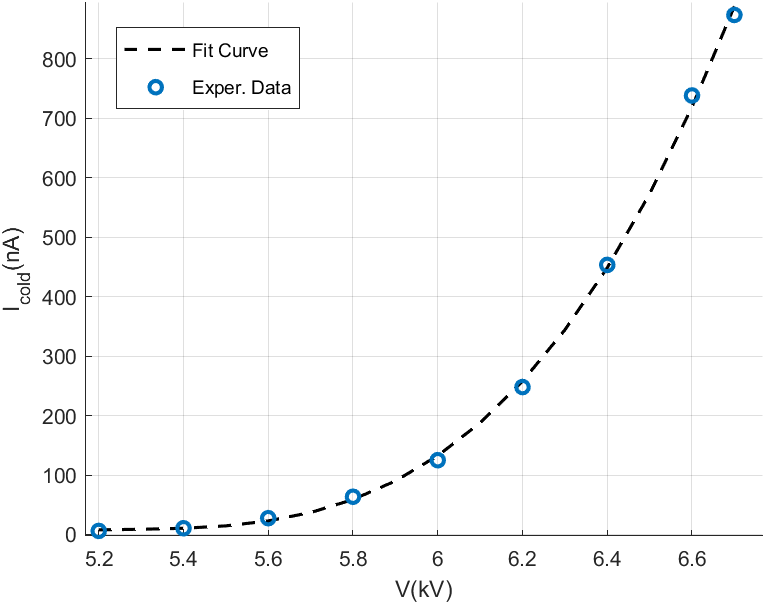
\includegraphics[scale=0.6]{IcoldV.png}
\end{figure}

Για να ελέγχθεί ο νόμος Fowler-Nordheim της σχέσης (\ref{13}), θέτουμε $X=1/V$ και $Y=ln\left[ I_{cold}/V^2\right]$ προκειμένου να τον γραμμικοποιήσουμε και να εφαρμόσουμε την μέθοδο των ελαχίστων τετραγώνων. Τότε ο νόμος παίρνει την μορφή 
\begin{align*}
Y&=lnC-B\cdot X \xRightarrow{D=lnC,G=-B	}\\ 
Y&=D+G\cdot X 				\numberthis
\end{align*}
Οι ποσότητες X, Y απ' τα πειραματικά δεδομένα φαίνονται στον Πίνακα 2. 
\begin{table}[h!]
\centering 
\caption{ }
\begin{tabular}{r|r|r|r}
$V(kV)$ & $I_{cold} (nA)$ & $X=1/V(kV^{-1})$ & $Y=ln(I_{cold}/V^2)$ \\ 
\hline\hline
10.5&  5.4&  0.1852&-1.0214 \\
27.5&  5.6&  0.1786&-0.1313\\
63.5&  5.8&  0.1724& 0.6353\\
  125.0&  6.0&  0.1667& 1.2448\\
  248.0&  6.2&  0.1613& 1.8643\\
  453.5&  6.4&  0.1563& 2.4044\\
  738.5&  6.6&  0.1515& 2.8305\\
  874.0&  6.7&  0.1493& 2.9689\\
\end{tabular}
\end{table}
 
 Με την μέθοδο ελαχίστων τετραγώνων προκύπτει η βέλτιστη ευθεία που προσεγγίζει τα δεδομένα σημεία $(X,Y)$ 
 \begin{align*}\label{18}
 Y=A+G\cdot X \text{ , όπου A=D=lnC=19.71 και G=-B=-111.21}\times10^3V  \numberthis
 \end{align*}
 \\
 Η γραφική παράσταση $Y=Y(X)$ φαίνεται στην  στην παρακάτω Εικόνα 4.
 
 \begin{figure}[h!]
 \centering
 \caption{ }
 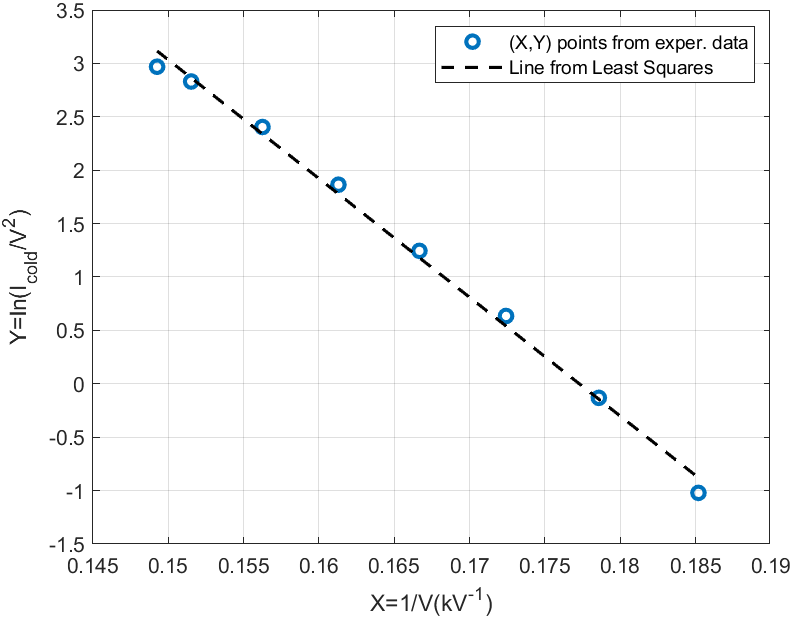
\includegraphics[scale=0.6]{least.png}
 \end{figure}
 
 Για να ολοκληρωθεί η μέθοδος ελαχίστων τετραγώνων μένει να υπολογισθεί το σφάλμα της κλίσης $\delta G$, για το οποίο έχουμε: 
 \begin{align*}
 \delta G&= \Delta G_{instr.} + \Delta G_{least sq.} \Rightarrow \\ 
 &= G\cdot\gamma_{V} + t_{n,p}\sqrt{\frac{1}{n\sum_k x_k^2-(\sum_k x_k)^2} \cdot \frac{\sum_k(y_k-A-Gx_k)^2}{n-2}} \Rightarrow \\ 
 &= 7.5627 \simeq 7.56 kV
 \end{align*}
 όπου $\gamma _V=3\%$ είναι το ποσοστιαίο σφάλμα που συνεισφέρουν τα όργανα στις τιμές των $X$ και $t_{n,p}=3.833$ η τιμή της κατανομής student για $n=8$ και $p\geq 99.7\%$.
 Άρα, τελικά έχουμε
 \begin{equation}
 G = (-111.21\pm7.56) kV
 \end{equation}
 
 Από την σχέση (\ref{14}) λύνοντας ως προς τον γεωμετρικό παράγοντα της ακίδας και θεωρώντας αναλλοίωτο το έργο εξαγωγής εξ' αιτίας του ηλεκτρικού πεδίου ($\phi=4.5eV)$ 
 %\textcolor{red}{και απ' την σχέση (\ref{18}) $C=e^{19.71}$ } 
έχουμε

 \begin{equation}
 \xi = \frac{6.83\times 10^9 \phi^{3/2}}{G} = 0.11\times10^6 m^{-1}
 \end{equation}
 
 
 το σφάλμα του προκύπτει από τη διάδοση του σφάλματος του G
 \begin{equation}
 \delta\xi = \sqrt{\left( \pdv{\xi}{G}\delta G \right)^2} = \frac{6.83\times10^9\phi^{3/2}}{G^2} \delta G = \frac{\xi}{G}\delta G=            0.00767\times10^6\simeq0.01\times10^6 m^{-1}
 \end{equation}

 Άρα έχουμε 
 \begin{equation} 
 \xi = (0.11\pm0.01 )\times10^6 m^{-1}
 \end{equation}
 Τώρα που έχουμε υπολογίσει τον γεωμετρικό παράγοντα της ακίδας, μπορούμε να υπολογίσουμε την ακτίνα της κορυφής λύνοντας την εξίσωση
 \begin{equation}
 \xi=\frac{1}{r}\frac{2}{ln(2R/r)} \Rightarrow \overbrace{\xi ln(2R/r) - \frac{2}{r}}^{f(r)} = 0 
 \end{equation}
 Η εξίσωση αυτή δεν λύνεται αναλυτικά και γι' αυτό θα προσεγγίσουμε τις λύσεις της χρησιμοποιώντας την επαναληπτική μέθοδο Newton-Raphson, $r_{n+1} = r_n-\frac{f(r_n)}{f'(r_n)}$ ξεκινώντας από την αρχική συνθήκη $r_0=0.001$ και χρησιμοποιώτας 10 επαναλήψεις. Η αρχική τιμή $r_0$ επιλέχθηκε τόσο μικρή διότι είναι αναμενόμενο η λύση να έχει μικρή τάξη μεγέθους $\mu m - mm$.Η λύση που προκύπτει είναι 
 \begin{align*}
 r = 1.64223\times10^{-6}  \Rightarrow \boxed{r \simeq 1.6\mu m}
 \end{align*}
 
 Τέλος, όταν η εφαρμοζόμενη τάση είναι ίση με $V_a = 5.2kV$, τότε από την σχέση (\ref{12}) μπορούμε να υπολογίσουμε το ηλεκτρικό πεδίο στην κορυφή της ακίδας 
 \begin{align*}
 F=\xi V_a\Rightarrow \boxed{F =586.7 MV/m}
 \end{align*}
\subsection*{Συμπεράσματα}
Γενικά, θεωρώ πως το πείραμα ήταν επιτυχημένο. Αυτό, διότι υπήρχε η αναπαραγωγή όλων των γνωστών θεωρητικών στοιχείων, όπως η εκθετική αύξηση του ρεύματος ψυχρής εκπομπής που επιβεβαίωσε το φαινόμενο σήραγγας και η ικανοποιητική ποιοτική συμφωνία των μετρήσεων με το μοντέλο Fowler-Nordheim (Εικόνα 4.).
\subsection*{Βιβιλιογραφία}
\begin{itemize}
\item[.] ΕΡΓΑΣΤΗΡΙΑΚΕΣ ΑΣΚΗΣΕΙΣ ΦΥΣΙΚΗΣ ΤΟΜΟΣ ΙΙ, ΣΥΛΛΟΓΙΚΟ
\item[.] Εισαγωγή στην Κβαντική Φυσική, Κωνσταντίνος Φαράκος, Γεώργιος Κουτσούμπας
\item[.] ΚΒΑΝΤΟΜΗΧΑΝΙΚΗ ΤΟΜΟΣ Ι, ΤΡΑΧΑΝΑΣ ΣΤΕΦΑΝΟΣ
\end{itemize}
\end{document}